\chapter{Active Registers}
\label{appendix:activeRegisters}

\begin{figure}
\centering{
\subfigure[1st Generation]{
\includegraphics[width=.4\columnwidth,height=.4\columnwidth,keepaspectratio=true]{./fig/RegisterGen1Front}
\label{fig:registerGen1}
}
\subfigure[2nd Generation]{
\includegraphics[width=.3\columnwidth,height=.3\columnwidth,keepaspectratio=true]{./fig/RegisterGen2Front}
\label{fig:registerGen2}
}
\subfigure[3rd Generation]{
\includegraphics[width=.3\columnwidth,height=.3\columnwidth,keepaspectratio=true]{./fig/RegisterGen3}
\label{fig:damper}
}
\subfigure[Bench-Top Test Rig]{
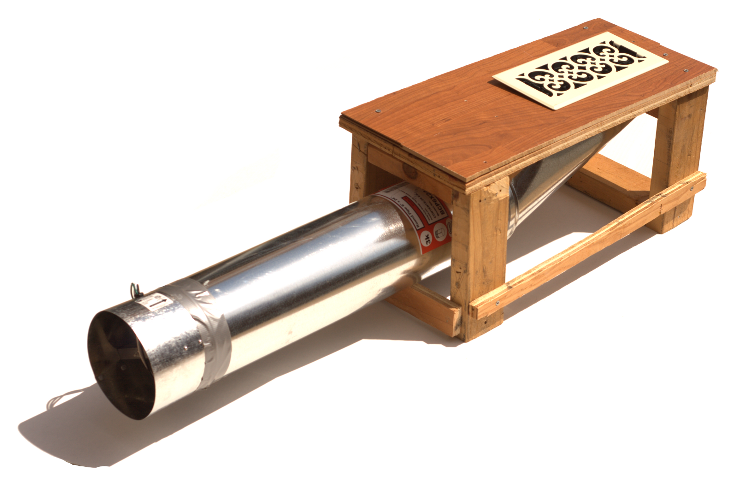
\includegraphics[width=.3\columnwidth,height=.3\columnwidth,keepaspectratio=true]{./fig/testRig}
\label{fig:testRig}
}
\caption[Three Generations of Active Registers and Bench-Top Test Rig]{(a)
Version 1 uses servo motors and a rotating louver design, but exhibited too much
leakage.  (b) Version 2 uses a sliding gate design to solve the leakage
problems, but causes too much noise.  (c) Version 3 is a commercial in-line
damper with a servo motor used for traditional zoning applications. (d) The
bench-top test rig used to verify that the second generation wirelessly
controlled active registers have almost no air leakage.}
\label{fig:activeRegisters}
}
\end{figure}

\begin{figure}
  \centering{
    \subfigure[Wireless Controller]{
    \includegraphics[width=.4\columnwidth]{./fig/registerBack}
      \label{fig:registerBack} }
    \subfigure[Face Plate of Active Register]{
    \includegraphics[width=.4\columnwidth]{./fig/registerFront}
    \label{fig:registerFront} } } \caption[Details of an active register]{A
    wirelessly controlled active register built by augmenting a standard vent
    register with a TelosB mote and a servo motor.} \label{fig:activeRegister}
\end{figure}




